\chapter{Service description and installation guide}

\section{Service description}
The service is an application that can classify objects in images (image classificator). The classification process runs separately from the web interface. Accordingly, the application is divided into a frontend and backend part.

\subsubsection{Frontend}
The frontend represents the web interface with which the user can perform various interactions such like upload images for the classification or to receive different forms of outputs. The web interface was developed using HTML, JavaScript and CSS. The website accepts images via an upload mechanism and then sends the image information to the backend where the classification process is performed in an extra Python file. In addition to this, Flask was used to enable the communication between JavaScript and Python. Flask is a lightweight web framework for Python which provides a simple way to create web applications by defining routes (URLs) and handling HTTP requests and responses \cite{Flask:2010}. After  the classification, the frontend receives the result as a JSON object. 

\subsubsection{Backend}
The backend is addressed via simple HTTP request. For image processing, the Python Imaging Library (PIL) is used to determine the many different image file formats that can be sent via the frontend. PIL provides a set of classes and methods for various image formats operations like reading, writing and also for image data manipulating such as cropping, rotation, and color conversions. For classification the Xception model from Keras is used. The Xception model is a trained convolutional neural network (CNN) model that recognizes and classifies images in the ImageNet dataset with high accuracy. The ImageNet dataset, contains over 1 million images and 1000 different classes \cite{Xception:2017}.

\section{Architecture}
    
    \begin{figure}[htbp]
        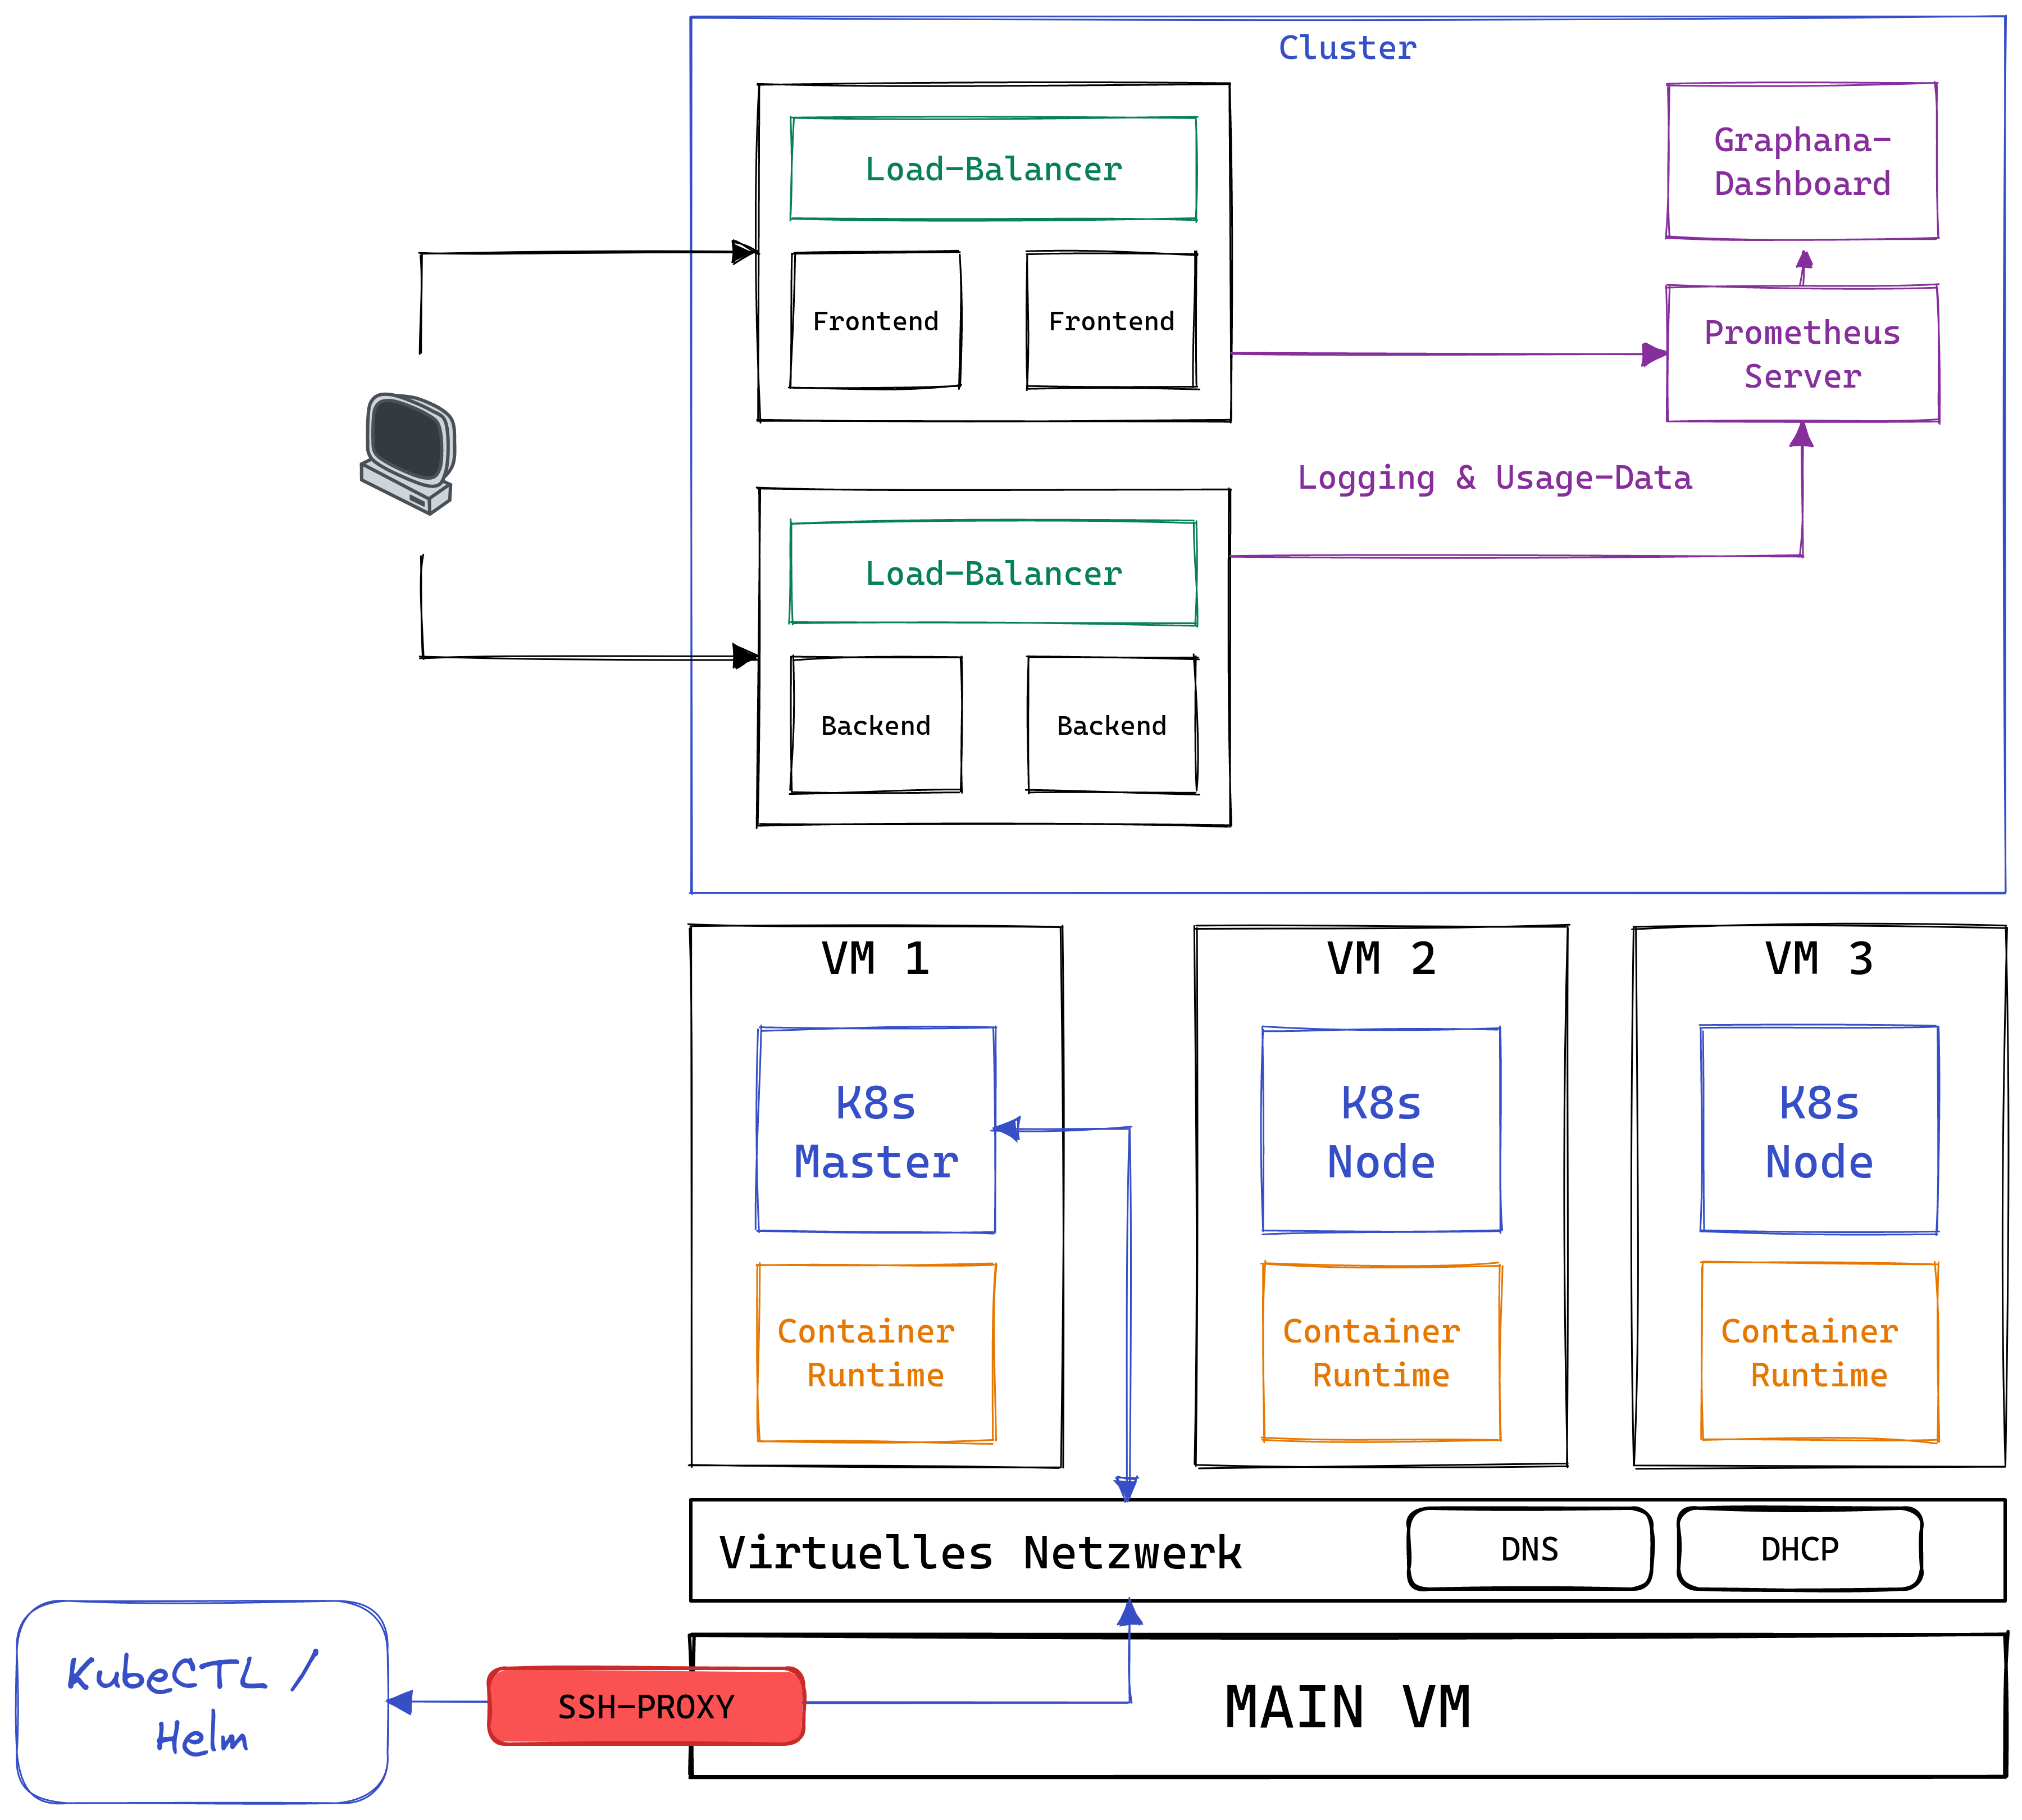
\includegraphics[width=15cm]{docs/assets/architecture-overview.png}
        \centering
        \captionsetup{justification=centering, margin=1cm}
        \caption{Architecture concept for the service deployment with Kubernetes}
        \label{fig:Architecture}
    \end{figure}

    In Figure~\ref{fig:Architecture} an overview of our proposed and afterwards implemented architecture for the service deployment and Kubernetes integration is shown. Therefore the function of the individual components are explained in detail as follows below.

\section{Application deployment}
    \subsection{Deployment Specifications}
        \subsubsection{Backend and Frontend}
            The deployment for the backend as well as the frontend is defined by the files \texttt{backend.yaml} and \texttt{frontend.yaml}.
            Once applied, it deploys a replica set consisting of three pods, build from the container image \texttt{zottelsheep/meds\_cloud:backend-\\latest} for the backend
            or \texttt{zottelsheep/meds\_cloud:frontend-latest} for the frontend and exposes the \texttt{containerPort 8000}.
            The services manage connections to these pods and make them available inside the cluster via the NodePort. 
            To specify which Pods should be addressed by the service, the \texttt{selector} field is used, which matches the tag from the deployed Pods.

        \subsubsection{Ingress}
            The ingress is used to make the services available to the outside of the cluster.
            It is described in \texttt{ingress.yaml}.
            Each service and its respective port are assigned an URL path, under which the resources can be accessed. 
        
    \subsection{Performing the Deployment}
        The command line tool \textbf{\texttt{kubectl}} is used for the application deployment.
        When managing a remote server, \texttt{kubectl} has to be configured, so that you can deploy from your machine.
        This is done with a \texttt{config} file, which should be located at \texttt{\$HOME\/.kube} or be specified with the \texttt{--kubeconfig} flag \cite{Kubernetes_kubeconfig:2022}.
        The \texttt{config} file specifies the server and proxy-url and also contains certificate data for a secure connection to the server.
        \medskip\\
        Once \texttt{kubectl} is configured and the cluster setup specified, deploying the application is simple.
        \begin{itemize}
            \item \texttt{kubectl apply -f backend.yaml} deploys the pods and service as defined in \texttt{backend.yaml}
            \item \texttt{kubectl apply -f frontend.yaml} deploys the pods and service as defined in \texttt{frontend.yaml}
            \item \texttt{kubectl apply -f ingress.yaml} deploys the ingress as defined in \texttt{ingress.yaml}
        \end{itemize}
        After the ingress is deployed, \texttt{kubectl get ingress} will list an external IP address.
        Using this IP address in combination with the paths defined in \texttt{ingress.yaml} , the services can be accessed either from a webbrowser or using a \texttt{curl} command.
    
\section{Usage}
After deploying everything correctly it is time to test it out. To do that you have to call \texttt{localhost} on port \texttt{8000}. There you can find our frontend where you can add a picture. You can do this in two different ways. You can either drag and drop the picture to the dedicated window or you can click on \texttt{Add Picture}. This will open an explorer where you can search and select your picture. After doing so you can see the five most likely categories and the associated probability.
